\subsection{Motivation}

Using the terminology in Section \ref{preliminaries}, we can express the notion of a \emph{closed} world in the current context. Specifically, the closed world assumption implies that $AP$, the set of atomic propositions with which LTL specifications are constructed from, is fixed. That is, if the robot encounters a new element of its world, which is not modeled as a proposition $\pi \in AP$, it will essentially ignore it, even if it is relevant to the mission.

Three main reasons motivate the need for open world mission specification and planning. First of all, in real-world applications, such as autonomous search and rescue scenarios, the mission is often specified before the robot has obtained full knowledge of the world. Second, the robot may have to incorporate new function and components to its strategy. Finally, the state-space may be too large for the user to enumerate every possible variation a priori.  To clarify these reasons, we introduce an illustrative example:

\begin{myExample}\label{Ex:mailbot1} Autonomous Mailbot (Fig. \ref{Fig:pr3})\\
	A robotic courier (mailbot) operates within a school or company building. It is tasked with collecting letters and delivering them to the recipients' offices. Even if all possible recipients, and the locations of their offices, are fixed, the information may not be available at the time the mission specification is defined.
\end{myExample}

\begin{figure}[ht]
	\centering
	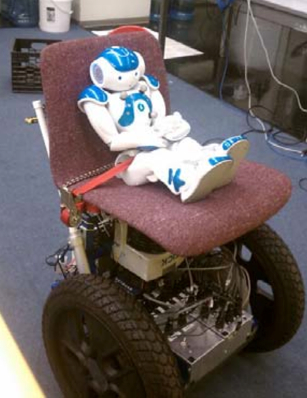
\includegraphics[width=0.7\columnwidth, clip]{./img/pr3.jpg}
	\caption{Our implementation of a mailbot. A Nao humanoid robot (ref ???) is mounted on a segway platform. The actuation and perception capabilities of the former are complemented by the localization, navigation and mobility advantages of the latter.}
	\label{Fig:pr3}
\end{figure}

In Example \ref{Ex:mailbot1}, notice that the robot does not operate serially, i.e., collecting one letter, delivering it, and returning for the next one. Rather, it is allowed to carry multiple letters at once, collect letters on its way to delivering a different letter, etc. Therefore, the specification must make sure that the robot only delivers letters at the correct location, that it is aware of which letters it is carrying, and that it does not forget to deliver a letter altogether. The open world aspect of the mission comes from the fact that new letters that correspond to new recipients may be collected by the robot during execution. Therefore, it is not possible to explicitly write a specification in the form of individual delivery tasks, e.g., \texttt{if you are sensing letter\_John\_Doe then do PickUp\_Letter and go to John\_Does\_office}. Notice that the detection of a letter addressed to a new recipient necessitates both its modeling, as a proposition, and the addition of another objective in the specification.

\subsection{Problem Statement}

We begin our formal analysis of the problem by defining a model of the open world, compatible with the current setting; that of controller synthesis.

Let $\W$ be a sequence of sets of atomic propositions:
\begin{equation}\label{Eq:W}
	\W = \left\{ AP_0, AP_1, \ldots, AP_k \right\}, \quad k \in \NN,
\end{equation} 
where $\mathcal{D} = \left\{ d_1, \ldots, d_m, \ldots, d_M \right\} \subseteq \mathcal{X}_k \subset AP_k, \forall k$. The abstract sensors in $\mathcal{D}$ are responsible for detecting $M$ types of new elements of the open world. For instance, one sensor $d$ may detect new letters, whereas another new offices.

In addition, let $A$ be a function which reads the sensors that environment propositions $\mathcal{D}$ abstract, and returns a new proposition if they detected an unmodeled element of the world:
\begin{equation}\label{Eq:A}
	A(m, k) = 
	\begin{cases}
		\left\{ \pi_{mk} \right\}, & \text{if } x_{d_m} \\ % Refers to valuation {0,1}
		\left\{ \right\}, &  \text{if } \neg x_{d_m}
	\end{cases}
\end{equation}�
where $x_{d_m} \in \Sigma_\mathcal{D}$ is the valuation of the $m$-th detection sensor, and $\pi_{mk} \not \in AP_k$. The new proposition $\pi_{mk}$ can be either an environment, or an action, or a region proposition.

Putting together Equations \eqref{Eq:W} -- \eqref{Eq:A}, we state our interpretation of an open world model.

\begin{myDefinition}\label{Def:openworld}	
	\textbf{(Open World Model):}
	The sequence $\W$ is an open world model if the sets $AP_k$ are iteratively defined:
	\begin{equation}\label{Eq:updateAP}
		AP_{k+1} = AP_k \bigcup_{m=1}^{M}A(m, k),
	\end{equation}
	and the index $k$ is then updated only if any of the $M$ detection sensors $\mathcal{D}$ become $\texttt{True}$:
	\begin{equation*}
		k \leftarrow 
		\begin{cases}
			k + 1, & \text{if } \bigvee_{m=1}^{M} x_{d_m} \\
			k, & \text{otherwise}
		\end{cases}
	\end{equation*}
	\end{myDefinition} 

We will return to this definition in Section \ref{openworld}, where we augment the update of the sets $AP_k$ in Eq. \eqref{Eq:updateAP} with additional new propositions.

In order to obtain a mission specification and a robot plan that can react to unmodeled elements of the world, we need to address two main problems. First of all, we should allow specifications that include formulas outside LTL, in order to allow ``self-adapting" missions (Problem \ref{Prob:newSpec}). Then, we need to define the specific mechanics of the new specification, which will allow new propositions $\pi_{mk} \in AP_{k+1}$ to be incorporated in LTL formulas (Sections \ref{abstractions}, \ref{openworld}).

The problem of rewriting a specification to allow for adding new propositions is formally stated below:

\begin{myProblem}\label{Prob:newSpec}
	\textbf{(Mission Specification Update):} Define a specification language $\Lambda$, and a parser $\mathcal{P}$ for it. Then, given a mission specification $\mathcal{M}$ written in $\Lambda$, a GR(1) formula $\varphi [k]$, and the latest set of atomic propositions $AP_{k+1}$, the LTL specification is updated:
	\begin{equation}\label{Eq:newSpec}
		\varphi [k+1] = \mathcal{P} (\mathcal{M}_{\varphi [k]}, AP_{k+1}),
	\end{equation}
	such that
	\begin{align*} % This is NOT right! The automaton has not been updated yet...
		x_{k+1} &\models \varphi_i^e [k+1], \; x_{k+1} \in \Sigma_{\mathcal{X}_{k+1}} = \Sigma_{\mathcal{X}_{k}} \cup \Sigma_{\mathcal{X}_{k+1} \backslash \mathcal{X}_{k}} \\
		y_{k+1} &\models \varphi_i^s [k+1], \; y_{k+1} \in \Sigma_{\mathcal{Y}_{k+1}} = \Sigma_{\mathcal{Y}_{k}} \cup \Sigma_{\mathcal{Y}_{k+1} \backslash \mathcal{Y}_{k}}
	\end{align*}
	% Also include a constraint on safeties and livenesses.
\end{myProblem}

The restrictions on $\varphi [k+1]$, the updated GR(1) specification, ensure that its initial conditions are compatible with the current ($k$) environment and robot state. Also, these restrictions set the values $x,y$ of any new propositions $\pi \in AP_{k+1} \backslash AP_{k}$. Furthermore, the notation $\mathcal{M}_{\varphi [k]}$ means that a subset of a mission specification $\mathcal{M}$ is equivalent to the GR(1) formula $\varphi[k]$. In other words $\mathcal{M}_{\varphi [k]}$ consists of a fixed part and a part that is updated when $\varphi[k]$ is updated.

Notice that the specification language $\Lambda$ and the parser $\mathcal{P}$ only provide the semantics and mechanics for updating $\varphi[k]$. The resulting formula, $\varphi [k+1]$, depends on the settings of the user-defined mission specification $\mathcal{M}$.

Given the problem statement above, we begin our definition of the new specification language $\Lambda$ with the notion of \emph{open world abstractions}. These abstractions allow us to specify tasks without explicitly referring to individual propositions. In Section \ref{abstractions} we show how they enable the systematic addition of new propositions to $AP_k$,  as well as the meaningful rewriting of $\varphi[k]$.

% END

%The first problem we aim to solve is a practical one. In a scenario such as that of Example \ref{Ex:mailbot1}, parts of the robot's state space (e.g. letters to carry) are potentially very large and could conceivably be expanded (or reduced) by the user in subsequent runs. To specify the same reactive behavior over an additional proposition in the domain, the user would have to modify or duplicate nearly every sentence in the specification. A more preferable approach would be to specify behaviors with an abstraction that does not explicitly refer to individual propositions.
%
%\begin{myProblem}\label{Prop:groups}
%	\textbf{(Specification Abstractions):}
%	Given a robot mission that includes indentical behavior over multiple propositions, express that mission in a specification language such that the individual propositions acted on identically are not explicitly referred to. 
%\end{myProblem}
%
%Our approach to Problem 1 is to include elements of first-order logic in our specification language, specifically set operations. We will first explain the theory and use of these abstractions in our specifications (Section \ref{abstractions}), and then apply them to the second part of our overall problem, updating an open world mission specification (Section \ref{openworld}). 